\newpage
\section{2019春}

\setcounter{yearcounter}{2019}
% \setcounter{page}{1}


\subsection{微分積分}
\prob{
  以下の境界値問題を解きなさい。
  \begin{enumerate}[label=(\alph*)]
    \item
    \begin{gather}
      \frac{dy}{dx} + \frac{1}{2}y = \frac{3}{2}
    \end{gather}
    \item
    \begin{gather}
      2x^2\frac{dy}{dx} + 3x\frac{dy}{dx} - y = 0
      \qquad 0\leq x \leq 1
      \quad y(0) = 0
      \quad y(1) = 1
    \end{gather}
  \end{enumerate}
}
\begin{ans*}
  ${}$
  \begin{enumerate}[label=(\alph*)]
    \item % [] 場合分け
    \begin{gather}
      \frac{1}{3-y}dy = \frac{1}{2}dx \\
      -\log|3-y| = \frac{1}{2}x + C \\
      y = Ae^{-\frac{x}{2}} + 3
    \end{gather}
    ただし、$C,\,A$は任意定数である。
    ここで、条件$y(0) = 2$より、
    \begin{gather}
      y(0) = A + 3 = 2 \\
      \therefore  A = -1
    \end{gather}
    ゆえに求める解は
    \begin{gather}
      y = -e^{-\frac{x}{2}} + 3
    \end{gather}
    \item Euler型より$x = e^t$とおく。このとき、
    \begin{align}
      \frac{dy}{dx}
        &= \frac{dy}{dt}\frac{dt}{dx} \\
        &= \frac{1}{x}\frac{dy}{dt} \\
      \frac{d^2y}{dx^2}
        &= \frac{d}{dx}\frac{dy}{dx} \\
        &= -\frac{1}{x^2}\frac{dy}{dt} + \frac{1}{x}\frac{d^2y}{dt^2}
    \end{align}
    より、与えられた微分方程式は次のようになる。
    \begin{align}
      2\frac{d^2y}{dt^2} + \frac{dy}{dt} - y = 0
    \end{align}
    補助方程式の解は\dm{\grl = \frac{1}{2},\,-1}であるので、一般解は任意定数$A,\,B$を用いて
    \begin{gather}
      y = Ae^{\frac{1}{2}t} + Be^{-t} \\
      \therefore y = A\sqrt{x} + \frac{B}{x}
    \end{gather}
  \end{enumerate}
\end{ans*}


\prob{
  次の積分を求めなさい。
  \begin{enumerate}[label=(\alph*)]
    \item
    \begin{gather}
      I_{1} = \int_{0}^{1}\int_{0}^{1} \max\{|x|,\,|y|\}\,dxdy
    \end{gather}
    \item
    \begin{gather}
      I_{2} = \iint_{D}(x^2+y)\,dxdy
      \qquad D = \Dset{(x,y)\in\mathcal{R}^2:|x|+|y|\leq 1}
    \end{gather}
  \end{enumerate}
}
\begin{ans*}
  ${}$
  \begin{enumerate}[label=(\alph*)]
    \item 下図のように領域$D_1,\,D_2$をおく。
    \begin{figure}[H]\centering
      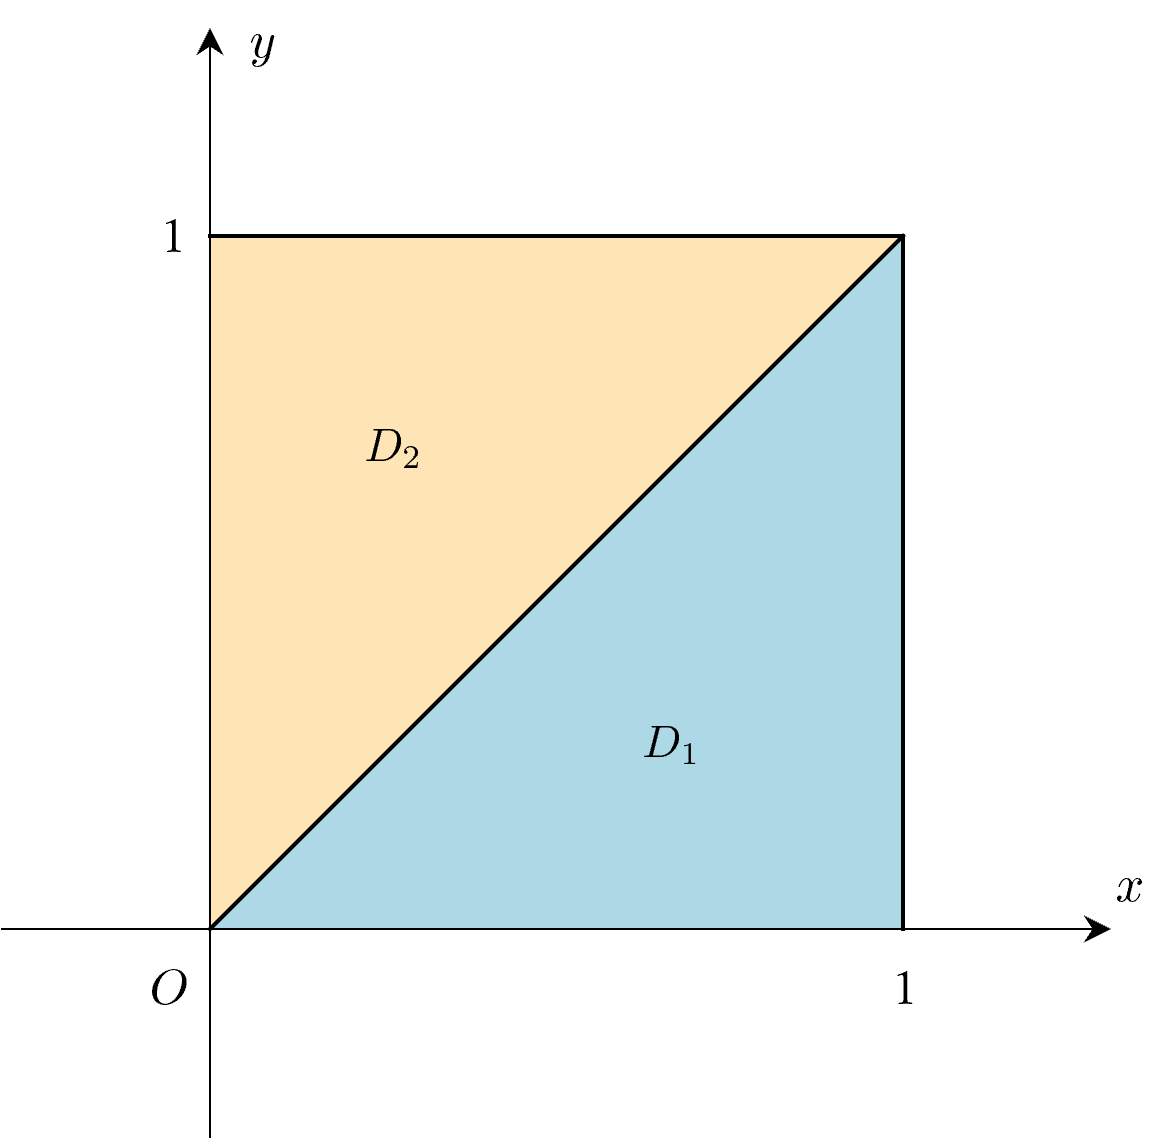
\includegraphics[width=.4\linewidth]{./src/fig/Basic/B_2019_spring_1-2-a.png}
    \end{figure}
    このとき、与えられた積分は
    \begin{gather}
      I_{1} = \int_{0}^{1}\int_{0}^{1} \max\{|x|,\,|y|\}\,dxdy
      = \iint_{D_1} x\,dxdy + \iint_{D_2}y\,dxdy
    \end{gather}
    と計算できる。
    よって、
    \begin{align}
      I_{1}
      &= \int_{0}^{1}\int_{0}^{x} x\,dydx + \int_{0}^{1}\int_{0}^{y} y\, dxdy \\
      &= \int_{0}^{1}x^2\,dx + \int_{0}^{1}y^2\,dy \\
      &= \frac{2}{3}
    \end{align}

    \item 与えられた積分において\dm{u = x + y,\,v = x - y}とおくと、
    \begin{gather}
      x = \frac{1}{2}(u+v) \\
      y = \frac{1}{2}(u-v) \\
      \ppar{x}{u} = \ppar{x}{v} = \ppar{y}{u} = \frac{1}{2} \\
      \ppar{y}{v} = -\frac{1}{2}
    \end{gather}
    より、ヤコビアン$J$は
    \begin{align}
      J
      &= \left|\frac{1}{2}\cdot\biggl(-\frac{1}{2}\biggr) - \frac{1}{2}\cdot\frac{1}{2}\right| \\
      &= \frac{1}{2}
    \end{align}
    である。よって、求める積分は
    \begin{align}
      I_2
      &= \int_{0}^{1}\int_{0}^{1}\frac{1}{2} \biggl(
        \frac{1}{4}(u+v)^2 + \frac{1}{2}(u-v)
      \biggr)\,dudv\\
      &= \int_{0}^{1}dv\left[\frac{1}{24}(u+v)^3 + \frac{1}{8}(u-v)^2\right]_{-1}^{1} \\
      &= \int_{0}^{1}
        \biggl(\frac{1}{24}(1+v)^3 + \frac{1}{8}(1-v)^2 - \frac{1}{24}(v-1)^3 - \frac{1}{8}(v+1)^2\biggr)
      \,dv \\
      &= \left[\frac{(1+v)^4}{96} - \frac{(1-v)^3}{24} - \frac{(v-1)^4}{96} - \frac{(v+1)^3}{24}\right]_{-1}^{1} \\
      &= \frac{1}{3}
    \end{align}
  \end{enumerate}
\end{ans*}




\subsection{線形代数}
\prob{
  次の行列$\bA$について、以下の問いに答えなさい。
  \begin{gather}
    \bA = \bmat{
      a & d & e \\
      0 & b & f \\
      0 & 0 & c
    }
  \end{gather}
  ここで、$a\neq 0,\,b\neq 0,\,c\neq 0$である。
  \begin{enumerate}[label=(\arabic*)]
    \item $\bA$は逆行列を持つことを証明しなさい。
    \item $\bA$の逆行列を求めなさい。
  \end{enumerate}
}
\begin{ans*}
  ${}$
  \begin{enumerate}[label=(\arabic*)]
    \item $\det\bA = abc\neq 0$より逆行列が存在する。
    \item $[\bA|\bE]$の行基本変形を考える。
    \begin{align}
      [\bA|\bE]
      &\lra \left[\begin{array}{ccc|ccc}
        1 & \frac{d}{a} & \frac{e}{a} & \frac{1}{a} & 0 & 0 \\
        0 & 1 & \frac{f}{b} & 0 & \frac{1}{b} & 0 \\
        0 & 0 & 1 & 0 & 0 & \frac{1}{c}
      \end{array}\right] \\
      &\lra \left[\begin{array}{ccc|ccc}
        1 & \frac{d}{a} & \frac{e}{a} & \frac{1}{a} & 0 & 0 \\
        0 & 1 & 0 & 0 & \frac{1}{b} & -\frac{f}{bc} \\
        0 & 0 & 1 & 0 & 0 & \frac{1}{c}
      \end{array}\right] \\
      &\lra \left[\begin{array}{ccc|ccc}
        1 & 0 & 0 & \frac{1}{a} & -\frac{d}{ab} & \frac{df - be}{abc} \\
        0 & 1 & 0 & 0 & \frac{1}{b} & -\frac{f}{bc} \\
        0 & 0 & 1 & 0 & 0 & \frac{1}{c}
      \end{array}\right]
    \end{align}
    より、逆行列は
    \begin{gather}
      \bA^{-1} = \bmat{
        \disp\frac{1}{a} & \disp-\frac{d}{ab} & \disp\frac{df - be}{abc} \\
        \\
        \disp 0 & \disp\frac{1}{b} & \disp-\frac{f}{bc} \\
        \\
        \disp 0 & \disp 0 & \disp \frac{1}{c}
      }
    \end{gather}
  \end{enumerate}
\end{ans*}


\prob{
  次の行列$\bA$について、以下の問いに答えなさい。
  \begin{gather}
    \bA = \bmat{
      1 & 1 & 0 \\
      0 & 2 & 1 \\
      0 & 0 & 3
    }
  \end{gather}
  \begin{enumerate}[label=(\arabic*)]
    \item $\bA$の階数(ランク)を求めなさい。
    \item $\bA$の固有値をすべて求めなさい。
    \item (2)で求めた固有値に対応する固有ベクトルをすべて求めなさい。ただし、大きさ1に正規化して答えなさい。
    \item $\bA$の対角化行列を求めなさい。
    \item (4)で求めた対角化行列の逆行列を求めなさい。
    \item $\bA$を対角化しなさい。
  \end{enumerate}
}
\begin{ans*}
  ${}$
  \begin{enumerate}[label=(\arabic*)]
    \item $\rank\bA = 3$
    \item 固有方程式より固有値$\grl$は
    \begin{gather}
      \det(\bA - \grl\bE) = (1-\grl)(2-\grl)(3-\grl) = 0 \\
      \therefore \grl = 3,\,2,\,1
    \end{gather}
    \item 固有ベクトルを$\bu = \{x,\,y,\,z\}^{\top}$とする。
    \begin{enumerate}[label=(\roman*)]
      \item $\grl = 3$のとき、
      \begin{gather}
        \bmat{
          -2 & 1 & 0 \\
          0 & -1 & 1 \\
          0 & 0 & 0
        }\Bmat{
          x \\ y \\ z
        } = \bzv \\
        \therefore
        \bu_{1} = \frac{1}{3}\Bmat{
          1 \\ 2 \\ 2
        }
      \end{gather}
      \item $\grl = 2$のとき、
      \begin{gather}
        \bmat{
          -1 & 1 & 0 \\
          0 & 0 & 1 \\
          0 & 0 & 1
        }\Bmat{
          x \\ y \\ z
        } = \bzv \\
        \therefore
        \bu_{2} = \frac{1}{\sqrt{2}}\Bmat{
          1 \\ 1 \\ 0
        }
      \end{gather}
      \item $\grl = 1$のとき、
      \begin{gather}
        \bmat{
          0 & 1 & 0 \\
          0 & 1 & 1 \\
          0 & 0 & 2
        }\Bmat{
          x \\ y \\ z
        } = \bzv \\
        \therefore
        \bu_{3} = \Bmat{
          1 \\ 0 \\ 0
        }
      \end{gather}
    \end{enumerate}
    \item この固有ベクトルの定数倍を列ベクトルとして持つ行列$\bP$は$\bA$を対角化する。
    \begin{gather}
      \bP = \bmat{
        1 & 1 & 1 \\
        2 & 1 & 0 \\
        2 & 0 & 0
      }
    \end{gather}
    \item 上の行列$\bP$の逆行列は$[\bP|\bE]$の行基本変形によって得る。
    \begin{align}
      [\bP|\bE]
      &\lra \left[\begin{array}{ccc|ccc}
        1 & 0 & 0 & 0 & 0 & \frac{1}{2} \\
        2 & 1 & 0 & 0 & 1 & 0 \\
        1 & 1 & 1 & 1 & 0 & 0
      \end{array}\right] \\
      &\lra \left[\begin{array}{ccc|ccc}
        1 & 0 & 0 & 0 & 0 & \frac{1}{2} \\
        0 & 1 & 0 & 0 & 1 & -1 \\
        0 & 0 & 1 & 1 & -1 & \frac{1}{2}
      \end{array}\right]
    \end{align}
    よって逆行列は
    \begin{gather}
      \bP^{-1} = \bmat{
        0 & 0 & \frac{1}{2} \\
        0 & 1 & -1 \\
        1 & -1 & \frac{1}{2}
      }
    \end{gather}
    \item $\bP^{-1}\bA\bP$が求める行列であり次のように対角化される。
    \begin{align}
      \bP^{-1}\bA\bP
      &= \bmat{
        0 & 0 & \frac{1}{2} \\
        0 & 1 & -1 \\
        1 & -1 & \frac{1}{2}
      }\bmat{
        1 & 1 & 0 \\
        0 & 2 & 1 \\
        0 & 0 & 3
      }\bmat{
        1 & 1 & 1 \\
        2 & 1 & 0 \\
        2 & 0 & 0
      } \\
      &= \bmat{
        0 & 0 & \frac{3}{2} \\
        0 & 2 & -2 \\
        1 & -1 & \frac{1}{2}
      }\bmat{
        1 & 1 & 1 \\
        2 & 1 & 0 \\
        2 & 0 & 0
      } \\
      &= \bmat{
        3 & 0 & 0 \\
        0 & 2 & 0 \\
        0 & 0 & 1
      }
    \end{align}
  \end{enumerate}
\end{ans*}



